\xiti
\begin{xiaotis}

\xiaoti{如图,三条直线相交于一点,任意找出图中的四对对顶角。}

\begin{figure}[htbp]
    \centering
    \begin{minipage}[b]{7cm}
        \centering
        \begin{tikzpicture}
    \tkzDefPoints{0/0/A, 4/0/B, 0.5/1/C, 3.5/-1/D, 0.8/-1.1/F, 3.2/1.1/E, 2/0/O}

    \tkzDrawSegments(A,B  C,D  E,F)
    \tkzLabelPoints[below](A, B, D, F, O)
    \tkzLabelPoints[left](C)
    \tkzLabelPoints[right](E)
\end{tikzpicture}


        \caption*{(第 1 题)}
    \end{minipage}
    \qquad
    \begin{minipage}[b]{7cm}
        \centering
        \begin{tikzpicture}
    \pgfmathsetmacro{\r}{2}
    \pgfmathsetmacro{\a}{35}
    \tkzDefPoints{0/0/O}
    \tkzDefPoint(180:\r){A}
    \tkzDefPoint(0:\r){B}
    \tkzDefPoint(180+\a:\r){C}
    \tkzDefPoint(\a:\r){D}
    \tkzDefPoint(180-\a:\r){E}

    \tkzDrawSegments(O,A  O,B  O,C  O,D  O,E)
    \tkzLabelPoints[below](B, C, D, O)
    \tkzLabelPoints[left](A, E)
\end{tikzpicture}


        \caption*{(第 3 题)}
    \end{minipage}
\end{figure}


\xiaoti{有公共顶点的两个角是对顶角吗?举例说明?}

\xiaoti{如图,已知直线 $AB$、$CD$ 相交于点 $O$, $OA$ 平分 $\angle EOC$,
    $\angle EOC = 70^\circ$,求 $\angle BOD$ 的度数。
}


\xiaoti{图中是对顶角量角器,试说明用它测量角度的原理。}

\begin{figure}[htbp]
    \centering
    \begin{minipage}[b]{7cm}
        \centering
        \includegraphics[width=5cm]{../pic/czjh1-ch2-xiti3-04.png}
        \caption*{(第 4 题)}
    \end{minipage}
    \qquad
    \begin{minipage}[b]{7cm}
        \centering
        \begin{tikzpicture}
    \tkzDefPoints{0/0/B,  3/0/C,  1/2/A,  2.5/2/D}

    \tkzDrawPolygon(A,B,C,D)
    \tkzLabelPoints[left](A, B)
    \tkzLabelPoints[right](C, D)
\end{tikzpicture}


        \caption*{(第 6 题)}
    \end{minipage}
\end{figure}

\xiaoti{任意画 $\angle AOB$, 再画 $\angle AOB$ 的平分线 $OC$。
    在射线 $OC$ 上任取一点 $P$, 画 $PD \perp OA$,$PE \perp OB$,
    垂足分别为 $D$、 $E$。用两脚规比较 $PD$ 和 $PE$ 的大小。
}

\xiaoti{如图。画 $AE \perp BC$、$CF \perp AD$(要延长 $AD$), 垂足分别为 $E$、$F$。}

\begin{figure}[htbp]
    \centering
    \begin{minipage}[b]{7cm}
        \centering
        \includegraphics[width=4cm]{../pic/czjh1-ch2-xiti3-07.png}
        \caption*{(第 7 题)}
    \end{minipage}
    \qquad
    \begin{minipage}[b]{7cm}
        \centering
        \begin{tikzpicture}
    \tkzDefPoints{0/0/B,  4/0/C,  1.6/2.5/A,  2.6/0/D}

    \tkzDrawPolygon(A,B,C)
    \tkzDrawSegment(A,D)
    \tkzLabelPoints[above](A)
    \tkzLabelPoints[left](B)
    \tkzLabelPoints[right](C)
    \tkzLabelPoints[below](D)
\end{tikzpicture}


        \caption*{(第 10 题)}
    \end{minipage}
\end{figure}


\xiaoti{要把水渠中的水引到水池 $C$, 在渠岸 $AB$ 的什么地方开沟,才能使沟最短?
    画出图来,并说明根据的是什么道理。
}

\xiaoti{画 $\angle AOB = 90^\circ$, 在边 $OA$ 上取一点 $C$, 使 $OC = 30\;\haomi$;
    在边 $OB$ 上取一点 $D$,使 $OD = 40\;\haomi$。
    经过点 $C$ 画 $OA$ 的垂线,经过点 $D$ 画 $OB$ 的垂线,两条垂线相交于点 $E$。
}
\begin{xiaoxiaotis}

    \xxt{量 $\angle CED$ 的度数(精确到 $1^\circ$);}

    \xxt{量点 $E$ 到 $OA$ 的距离、点 $E$ 到 $OB$ 的距离、
         点 $E$ 到点 $O$ 的距离、点 $C$ 到点 $D$ 的距离(精确到 $1\;\haomi$)。
    }

\end{xiaoxiaotis}

\xiaoti{画线段 $AB = 48\;\haomi$, 再画线段 $AB$ 的中垂线 $MN$。
    在 $MN$ 上取两点 $C$、$D$,使点 $C$ 到 $AB$ 的距离、点 $D$ 到 $AB$ 的距离
    分别等于 $18\;\haomi$、$32\;\haomi$。量出 $AC$、$BC$、$AD$、$BD$ 的长度
    (精确到 $1\;\haomi$),并比较它们的大小。
}

\xiaoti{用三角板,过点 $B$、$C$ 分别画 $AD$ 的垂线;过点 $B$ 分别画 $AC$、$AB$ 的垂线。}


\xiaoti{图甲、图乙、图丙中的 $\angle 1$ 和 $\angle 2$, $\angle 3$ 和 $\angle 4$
    各是哪两条直线被哪一条直线所截而成的?它们各是什么角?
}

\begin{figure}[htbp]
    \centering
    \begin{minipage}[b]{5.0cm}
        \centering
        \begin{tikzpicture}[scale=0.9]
    \tkzDefPoints{0/0/B,  3/0/C,  2/2/A,  4.2/0/D, 4/2/E}

    \tkzDrawSegments(B,D  B,A  A,C  C,E)
    \tkzMarkAngle[size=0.6](D,C,E)    \tkzLabelAngle[pos=0.9](D,C,E){$1$}
    \tkzMarkAngle[size=0.4](C,B,A)    \tkzLabelAngle[pos=0.7](C,B,A){$2$}
    \tkzMarkAngle[size=0.4](E,C,A)    \tkzLabelAngle[pos=0.7](E,C,A){$3$}
    \tkzMarkAngle[size=0.4](B,A,C)    \tkzLabelAngle[pos=0.7](B,A,C){$4$}

    \tkzLabelPoints[above](A)
    \tkzLabelPoints[left](B)
    \tkzLabelPoints[right](E)
    \tkzLabelPoints[below](C,D)
\end{tikzpicture}


        \caption*{甲}
    \end{minipage}
    \qquad
    \begin{minipage}[b]{4.5cm}
        \centering
        \begin{tikzpicture}[scale=0.9]
    \tkzDefPoints{0/0/A,  3/0/B,  3.8/2/C,  0.8/2/D}

    \tkzDrawPolygon(A,B,C,D)
    \tkzDrawSegments(B,D)
    \tkzMarkAngle[size=0.6](B,D,C)    \tkzLabelAngle[pos=0.9](B,D,C){$1$}
    \tkzMarkAngle[size=0.6](D,B,A)    \tkzLabelAngle[pos=0.9](D,B,A){$2$}
    \tkzMarkAngle[size=0.4](A,D,B)    \tkzLabelAngle[pos=0.7](A,D,B){$3$}
    \tkzMarkAngle[size=0.4](C,B,D)    \tkzLabelAngle[pos=0.7](C,B,D){$4$}

    \tkzLabelPoints[above](D,C)
    \tkzLabelPoints[below](A,B)
\end{tikzpicture}


        \caption*{乙}
    \end{minipage}
    \begin{minipage}[b]{4.5cm}
        \centering
        \begin{tikzpicture}[scale=0.9]
    \tkzDefPoints{0/0/A,  3/0/B,  3.8/2/C,  0.8/2/D,  4.2/0/E}

    \tkzDrawPolygon(A,B,C,D)
    \tkzDrawSegments(B,E)
    \tkzMarkAngle[size=0.4](D,C,B)    \tkzLabelAngle[pos=0.7](D,C,B){$1$}
    \tkzMarkAngle[size=0.4](C,B,A)    \tkzLabelAngle[pos=0.7](C,B,A){$2$}
    \tkzMarkAngle[size=0.6](B,A,D)    \tkzLabelAngle[pos=0.9](B,A,D){$3$}
    \tkzMarkAngle[size=0.6](E,B,C)    \tkzLabelAngle[pos=0.9](E,B,C){$4$}

    \tkzLabelPoints[above](D,C)
    \tkzLabelPoints[below](A,B,E)
\end{tikzpicture}


        \caption*{丙}
    \end{minipage}
    \caption*{(第 11 题)}
\end{figure}


\xiaoti{图中,下列各对角分别是什么角?}
\begin{xiaoxiaotis}

    \xxt{$DE$ 和 $BC$ 被 $AB$ 所截而得的 $\angle ADE$ 和 $\angle B$,被 $AC$ 所截而得的 $\angle C$ 和 $\angle DEC$;}

    \xxt{$AB$ 和 $AC$ 被 $BC$ 所截而得的 $\angle B$ 和 $\angle C$, 被 $DE$ 所截而得的 $\angle ADE$ 和 $\angle DEC$。}

\end{xiaoxiaotis}

\begin{figure}[htbp]
    \centering
    \begin{minipage}[b]{7cm}
        \centering
        \begin{tikzpicture}
    \tkzDefPoints{0/0/B,  3/0/C,  1.5/2/A}
    \tkzDefPointOnLine[pos=0.4](A,B)  \tkzGetPoint{D}
    \tkzDefPointOnLine[pos=0.6](A,C)  \tkzGetPoint{E}

    \tkzDrawPolygon(A,B,C)
    \tkzDrawSegments(D,E)

    \tkzLabelPoints[above](A)
    \tkzLabelPoints[left](D)
    \tkzLabelPoints[right](E)
    \tkzLabelPoints[below](B,C)
\end{tikzpicture}


        \caption*{(第 12 题)}
    \end{minipage}
    \qquad
    \begin{minipage}[b]{7cm}
        \centering
        \begin{tikzpicture}
    \tkzDefPoints{0/0/B,  3/0/C,  1.5/1.5/A, 2.8/2/D}
    \tkzDefPointOnLine[pos=1.6](B,A)  \tkzGetPoint{E}

    \tkzDrawPolygon(A,B,C)
    \tkzDrawSegments(A,E  A,D)
    \tkzMarkAngle[size=0.5](D,A,E)    \tkzLabelAngle[pos=0.8](D,A,E){$1$}
    \tkzMarkAngle[size=0.3](C,A,D)    \tkzLabelAngle[pos=0.5](C,A,D){$2$}

    \tkzLabelPoints[left](A)
    \tkzLabelPoints[right](E)
    \tkzLabelPoints[below](B,C,D)
\end{tikzpicture}


        \caption*{(第 13 题)}
    \end{minipage}
\end{figure}

\xiaoti{图中 $\angle 1$ 和 $\angle B$ 是不是同位角,$\angle 2$ 和 $\angle B$ 呢?
    $\angle EAC$ 与 $\angle B$ 呢?为什么?
}

\end{xiaotis}

